\section{Network Diagram}
\label{sec:diagram}

\subsection{Description}

A full diagram of BT network is shown in Figure \ref{fig:diagram}.
There are 3 routers in the network, whose names are BT-R001, BT-R002 and BT-R003 resepectively, connected to each other. 
Each connection forms a Router-Router subnet with only 2 interfaces.

On the other hand, each router is connected with a laptop separately named as BT001, BT002 and BT003 and thus forms a Router-Laptop subnet.
A customer of BT Network is assigned with a Router-Laptop subnet and has a minimum of 10 host IP addresses.

To connect to neighbouring ISPs, a Router-Neighbour subnet is formed for each connection. Concretely, Router 2 (BT-R002) is connected to one of DT Network's routers while Router 3 (BT-R003) is connected to one of Virgin Network's and Central Network's routers separately.

All of the above connections are through physical cables.

\begin{landscape}
\begin{figure}[t!]
    \centering
    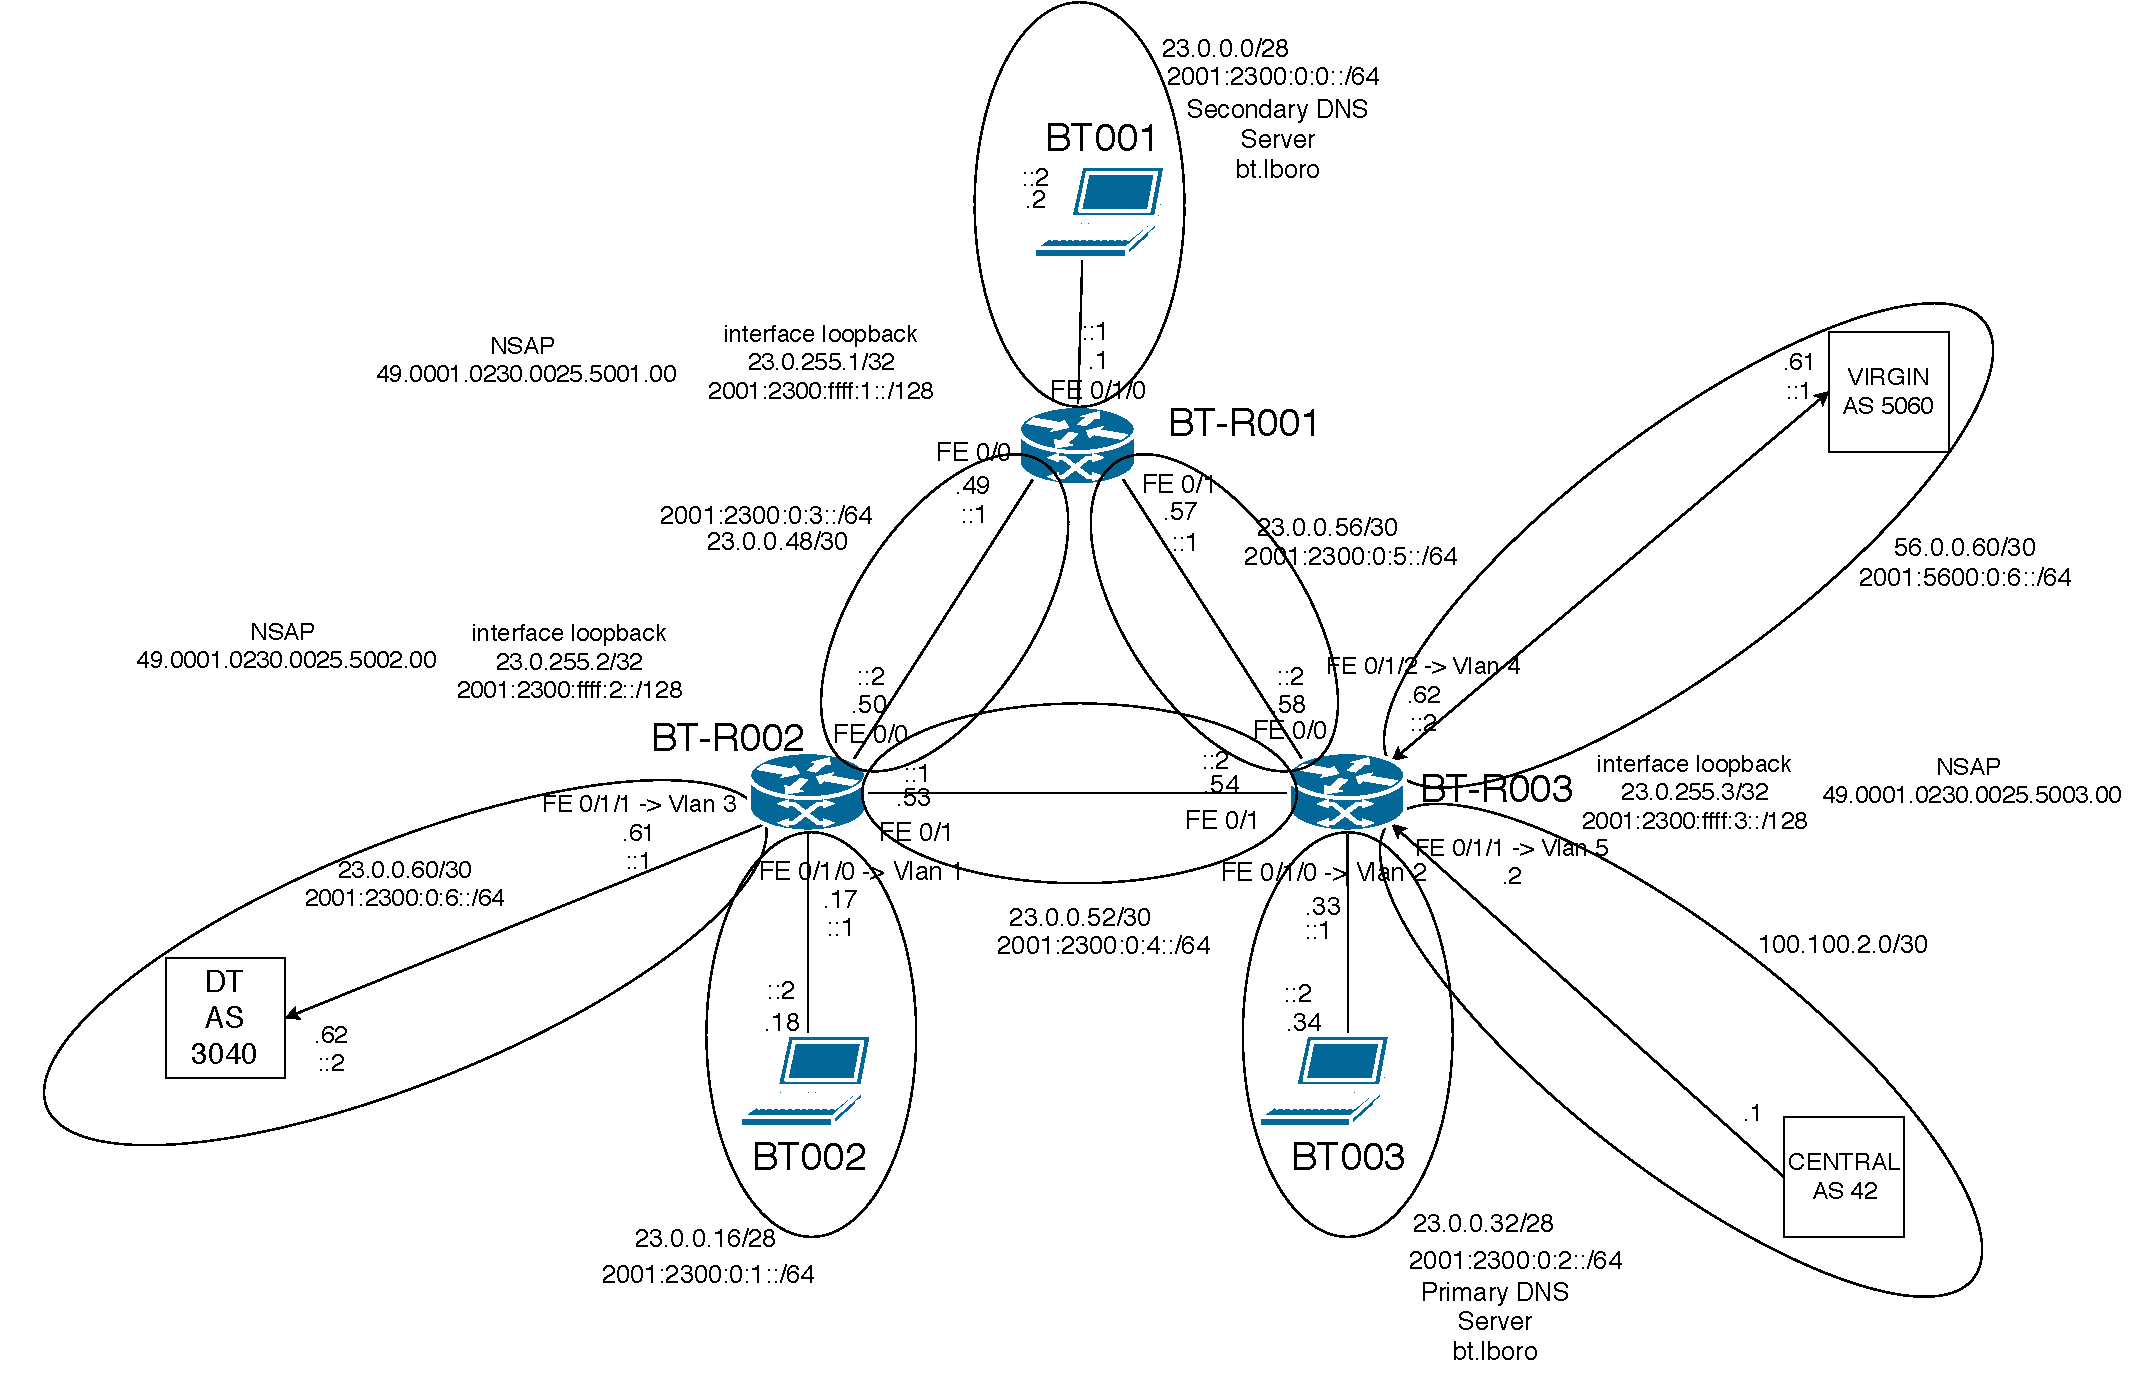
\includegraphics[width=\linewidth]{diagram}
    \caption{Full Network Diagram of BT Network.}
    \label{fig:diagram}
\end{figure}
\end{landscape}




\subsection{IP Addresses and Interfaces}

An IPv4 address range of \texttt{23.0.0.0/8} and IPv6 address range of \texttt{2001:2300::/32} are allocated to BT Network, which are further divided into sub-ranges to be allocated to each subnet.

For IPv4 addressing, a prefix of $n$ is needed for a subnet that demands $X$ host addresses, where $n$ is an integer that satisfies $2^{32-n} - 2 \geq X$ and $n \leq 32$. For our lab, the maximum value for prefix is used in order to minimize the size of each subnet and reserve address space for future customers. 
\textbf{However, it's also possible to use a larger value for each Router-Laptop subnet in order to maximize the size of the subnet, given that the number of customers (in this case, $3$) is fixed.}

In BT Network, the prefix for each Router-Router and Router-Neighbour subnet is $30$ while the prefix for each Router-Laptop subnet is $28$. In other words, each Router-Router and Router-Neighbour subnet has $2$ guaranteed IPv4 host addresses while each Router-Laptop subnet has $14$ guaranteed IPv4 host addresses. During address block allocation, larger subnet is being considered before smaller one reduce the number of block segments.

For IPv6 addressing, however, each subnet has a fixed prefix of $64$ to ensure that each interface in the subnet has a unique address. The full details of IP address allocation is shown in Table \ref{tab:ip}.

\begin{figure}[ht!]
    \centering
    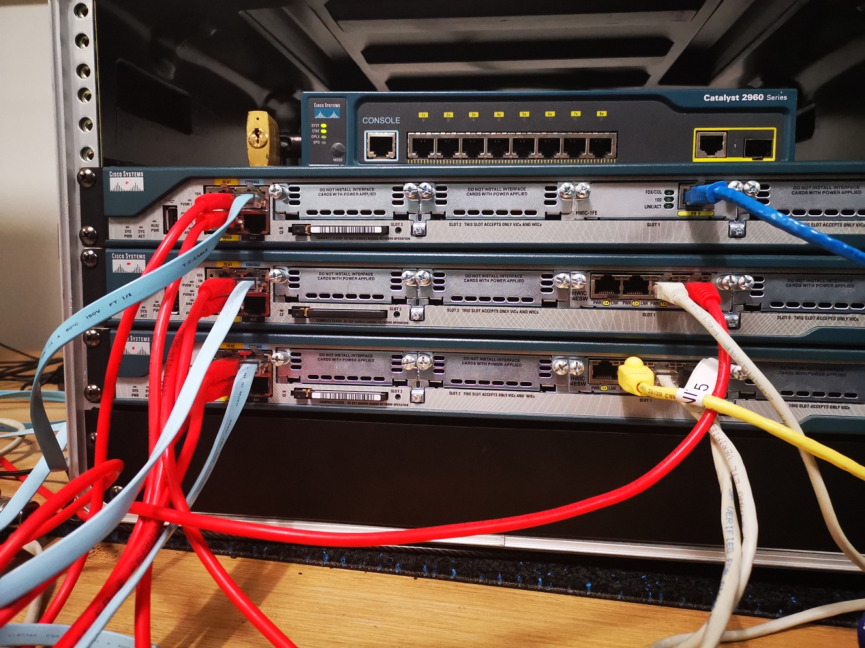
\includegraphics[width=0.8\linewidth]{physical}
    \caption{Physical Connections within BT Network.}
    \label{fig:physical}
\end{figure}

In terms of interfaces, there are $3$ Ethernet interfaces (\texttt{FastEthernet0/0}, \texttt{FastEthernet0/1} and \texttt{FastEthernet0/1/0}) on Router 1, each of which can be assigned with an IP address. On Router 2 and 3, however, there are $6$ Ethernet interfaces each and only $2$ of them (\texttt{FastEthernet0/0} and \texttt{FastEthernet0/1}) can be directly assigned with IP addresses. 
The remaining $4$ interfaces are link layer interfaces and thus does not possess any IP address.
To be assigned with an IP address, such an interface need to be assigned to an Virtual LAN (VLAN) to which the address is actually assigned.

Router-Router connections are established through either \texttt{FastEthernet0/0} or \texttt{FastEthernet0/1} interfaces on both ends while Router-Laptop and Router-Neighbour are through one of the remaining interfaces on the router end.
Since both interfaces are on the left-hand side of each router and such arrangement helps distinguishing between Router-Router connections and others easily as shown in Figure \ref{fig:physical}. Interfaces of both ends for each connection as well as their corresponding IP addresses are detailed in Table \ref{tab:interfaces}.

\begin{landscape}
\scriptsize{
\begin{longtable}[]{@{}lllll@{}}
\toprule
Subnet & IPv4 Address / Prefix & IPv4 Address Range & IPv6
Address / Prefix & IPv6 Address Range\tabularnewline
\midrule
\endhead
\texttt{BT-R001} - \texttt{BT001} & \texttt{23.0.0.0/28} &
\texttt{23.0.0.1} - \texttt{23.0.0.14} & \texttt{2001:2300:0:0::/64} &
\texttt{2001:2300:0:0::1} -
\texttt{2001:2300:0:0:ffff:ffff:ffff:fffe}\tabularnewline
\texttt{BT-R002} - \texttt{BT002} & \texttt{23.0.0.16/28} &
\texttt{23.0.0.17} - \texttt{23.0.0.30} & \texttt{2001:2300:0:1::/64} &
\texttt{2001:2300:0:1::1} -
\texttt{2001:2300:0:1:ffff:ffff:ffff:fffe}\tabularnewline
\texttt{BT-R003} - \texttt{BT003} & \texttt{23.0.0.32/28} &
\texttt{23.0.0.33} - \texttt{23.0.0.62} & \texttt{2001:2300:0:2::/64} &
\texttt{2001:2300:0:2::1} -
\texttt{2001:2300:0:2:ffff:ffff:ffff:fffe}\tabularnewline
\texttt{BT-R001} - \texttt{BT-R002} & \texttt{23.0.0.48/30} &
\texttt{23.0.0.49} - \texttt{23.0.0.50} & \texttt{2001:2300:0:3::/64} &
\texttt{2001:2300:0:3::1} -
\texttt{2001:2300:0:3:ffff:ffff:ffff:fffe}\tabularnewline
\texttt{BT-R002} - \texttt{BT-R003} & \texttt{23.0.0.52/30} &
\texttt{23.0.0.53} - \texttt{23.0.0.54} & \texttt{2001:2300:0:4::/64} &
\texttt{2001:2300:0:4::1} -
\texttt{2001:2300:0:4:ffff:ffff:ffff:fffe}\tabularnewline
\texttt{BT-R001} - \texttt{BT-R003} & \texttt{23.0.0.56/30} &
\texttt{23.0.0.57} - \texttt{23.0.0.58} & \texttt{2001:2300:0:5::/64} &
\texttt{2001:2300:0:5::1} -
\texttt{2001:2300:0:5:ffff:ffff:ffff:fffe}\tabularnewline
\texttt{BT-R002} - \texttt{DT} & \texttt{23.0.0.60/30} &
\texttt{23.0.0.61} - \texttt{23.0.0.62} & \texttt{2001:2300:0:6::/64} &
\texttt{2001:2300:0:6::1} -
\texttt{2001:2300:0:6:ffff:ffff:ffff:fffe}\tabularnewline
\texttt{BT-R003} - \texttt{Virgin} & \texttt{56.0.0.60/30} &
\texttt{56.0.0.61} - \texttt{56.0.0.62} & \texttt{2001:5600:0:6::/64} &
\texttt{2001:5600:0:6::1} -
\texttt{2001:5600:0:6:ffff:ffff:ffff:fffe}\tabularnewline
\texttt{BT-R003} - \texttt{Central} & \texttt{100.100.2.0/30} &
\texttt{100.100.2.1} - \texttt{100.100.2.2} & &\tabularnewline
\bottomrule
\caption{Allocation of IPv4 and IPv6 Addresses to Subnets in BT Network.}
\label{tab:ip}
\end{longtable}
}

\scriptsize{
\begin{longtable}[]{@{}lllllll@{}}
\toprule
Connection & Interface 1 & IPv4 Address & IPv6 Address & Interface 2 & IPv4 Address & IPv6
Address \tabularnewline
\midrule
\endhead
\texttt{BT-R001} - \texttt{BT001} & \texttt{BT-R001}:
\texttt{FastEthernet0/1/0} & \texttt{23.0.0.1} &
\texttt{2001:2300:0:0::1} & \texttt{BT001}: \texttt{eth0} &
\texttt{23.0.0.2} & \texttt{2001:2300:0:0::2}\tabularnewline
\texttt{BT-R002} - \texttt{BT002} & \texttt{BT-R002}:
\texttt{FastEthernet0/1/0} -\textgreater{} \texttt{Vlan\ 1} &
\texttt{23.0.0.17} & \texttt{2001:2300:0:1::1} & \texttt{BT002}:
\texttt{eth0} & \texttt{23.0.0.18} &
\texttt{2001:2300:0:1::2}\tabularnewline
\texttt{BT-R003} - \texttt{BT003} & \texttt{BT-R003}:
\texttt{FastEthernet0/1/0} -\textgreater{} \texttt{Vlan\ 2} &
\texttt{23.0.0.33} & \texttt{2001:2300:0:2::1} & \texttt{BT003}:
\texttt{eth0} & \texttt{23.0.0.34} &
\texttt{2001:2300:0:2::2}\tabularnewline
\texttt{BT-R001} - \texttt{BT-R002} & \texttt{BT-R001}:
\texttt{FastEthernet0/0} & \texttt{23.0.0.49} &
\texttt{2001:2300:0:3::1} & \texttt{BT-R002}: \texttt{FastEthernet0/0} &
\texttt{23.0.0.50} & \texttt{2001:2300:0:3::2}\tabularnewline
\texttt{BT-R002} - \texttt{BT-R003} & \texttt{BT-R002}:
\texttt{FastEthernet0/1} & \texttt{23.0.0.53} &
\texttt{2001:2300:0:4::1} & \texttt{BT-R003}: \texttt{FastEthernet0/1} &
\texttt{23.0.0.54} & \texttt{2001:2300:0:4::2}\tabularnewline
\texttt{BT-R001} - \texttt{BT-R003} & \texttt{BT-R001}:
\texttt{FastEthernet0/1} & \texttt{23.0.0.57} &
\texttt{2001:2300:0:5::1} & \texttt{BT-R003}: \texttt{FastEthernet0/0} &
\texttt{23.0.0.58} & \texttt{2001:2300:0:5::2}\tabularnewline
\texttt{BT-R002} - \texttt{DT} & \texttt{BT-R002}:
\texttt{FastEthernet0/1/1} -\textgreater{} \texttt{Vlan\ 3} &
\texttt{23.0.0.61} & \texttt{2001:2300:0:6::1} & \texttt{DT} &
\texttt{23.0.0.62} & \texttt{2001:2300:0:6::2}\tabularnewline
\texttt{BT-R003} - \texttt{Virgin} & \texttt{BT-R003}:
\texttt{FastEthernet0/1/2} -\textgreater{} \texttt{Vlan\ 4} &
\texttt{56.0.0.62} & \texttt{2001:5600:0:6::2} & \texttt{Virgin} &
\texttt{56.0.0.61} & \texttt{2001:5600:0:6::1}\tabularnewline
\texttt{BT-R003} - \texttt{Central} & \texttt{BT-R003}:
\texttt{FastEthernet0/1/1} -\textgreater{} \texttt{Vlan\ 5} &
\texttt{100.100.2.2} & & \texttt{Central} & \texttt{100.100.2.1}
&\tabularnewline
\bottomrule
\caption{Interfaces for Each Physical Connection and Corresponding IPv4 and IPv6 Addresses.}
\label{tab:interfaces}
\end{longtable}
}

\end{landscape}






